\section{Bevezetés}
\index{GtkWindow@\texttt{GtkWindow}}
\index{GtkDialog@\texttt{GtkDialog}}

Ebben a részében a \textit{GTK}-ban létrehozható különböző ablaktípusok közös vonásait, valamint az eltéréseik okait vesszük sorra. Kitérünk egyrészről az egyes ablaktípusok létrehozásának sajátosságaira, azok \textit{widget}ekkel való feltöltésére, másrészről a felhasználó interakciók kezelésére, ezzel együtt az ablakok bezárásának módjaira is, szem előtt tartva természetese a \textit{C}, illetve a \textit{C++} nyelvű változat azonosságait, különbözőségeit.

\subsection{\textit{Popup} és \textit{toplevel} ablakok}
\label{sec:windowtype}

A \textit{popup} ablakra, mint típusra ugyan ritkán lesz közvetlenül szükségünk, érdemes tudni, hogy a \textit{GTK} -- mint látszik -- ebben a tekintetben két fajta ablakot különböztet meg. A \textit{popup}\index{ablak!típus!popup}\index{GtkWindow@\texttt{GtkWindow}!tulajdonságok!type@\texttt{type}} (felugró, felbukkanó) ablakokat, melyekre -- valamilyen speciális célt szolgáló saját készítésű \textit{widget}ektől eltekintve -- csak néhány példa létezik (\textit{menu}, \textit{tooltip}), valamint a \textit{toplevel}\index{ablak!típus!toplevel} (legkülső, legfelső szintű) ablakokat, melyek csaknem minden \textit{GTK}-s, illetve saját fejlesztésű ablak alapjául szolgálnak. Ha tehát az ablakra, illetve a hozzá kapcsolódó fogalmakra gondolunk, többségében egy \textit{toplevel} ablakra gondolunk, és nem a \textit{popup}\footnote{Más eszközkészletek a ``popups'' gyűjtőfogalom alá sorolják a dialógusokat, a \textit{GTK} esetén azonban egy dialógus ablak mindig egy \textit{toplevel}} típusúakra, melyekről talán nem is feltételeznénk első ránézésre, hogy ablakok.

Az ablakkezelő ezt az információt használja fel annak eldöntésére, hogy az adott ablakot milyen kerettel, dekorációval lássa el, illetve általánosságban menedzselje e a konkrét ablakot. Utóbbi -- azaz a \textit{toplevel}\index{GtkWindow@\texttt{GtkWindow}!tulajdonságok!type@\texttt{type}} ablakok -- esetben alapértelmezetten az ablakkezelő keretet, illetve a beállításoktól függően azon például bezáró, teljes mértre váltó, minimalizáló gombot jelenít meg. A \textit{popup} típusú ablakokat az ablakkezelő nemcsak hogy nem dekorálja, de nem is menedzseli, következésképp tehát számos -- az ablakkezelő hatáskörébe tartozó -- funkció, mint amilyen például a minimalizálás, vagy a maximalizálás nem is érhető el. Bár kézenfekvő megoldásnak látszik a \textit{popup} típus arra, ha egy dekoráció nélküli ablakot készítsünk, mégse ezt tegyük, az ilyen típusú megjelenésbeli sajátosságok beállítására léteznek külön függvények.

Minden \textit{window} egyben konténer is, pontosabban fogalmazva egy \textit{bin}\index{GtkBin@\texttt{GtkBin}}, azaz nem túl meglepő módon tartalmazhat egy további elemet gyerekként, ami természetesen szintén lehet egy konténer, így biztosítva, hogy számos elemet helyezhessünk el az elkészített ablakon belül.

\subsection{\textit{Window} és \textit{dialóg}}
\index{GtkWindow@\texttt{GtkWindow}}
\index{GtkDialog@\texttt{GtkDialog}}
\index{GtkBox@\texttt{GtkBox}!függvények!pack\_end@\texttt{pack\_end}}
\index{GtkBox@\texttt{GtkBox}!függvények!pack\_start@\texttt{pack\_start}}

\label{par:dialogbox}
A \textit{window} típus -- azon belül is ahogy tárgyaltuk a \textit{toplevel window}\index{ablak!típus!toplevel} -- közvetlen szülője a \textit{dialog} típusnak, számottevő különbség tulajdonképpen nincs is a kettő között. Egy \textit{dialog} nem más, mint egy olyan \textit{window}, melybe a \textit{GTK+} fejlesztői néhány hasznos elemet helyeztek el. Konkrétabban fogalmazva minden dialógba egy függőleges elrendezésű konténer \textit{widget} (\textit{VBox}\index{GtkVBox@\texttt{GtkVBox}}), abba pedig egy, a gombok elhelyezésére szolgáló konténer (\textit{HButtonBox} típusú \texttt{action\_area}\index{GtkDialog@\texttt{GtkDialog}!belső elemek!action\_area@\texttt{action\_area}}), valamint egy szeparátor (\textit{HSpearator\index{GtkHSeparator@\texttt{GtkHSeparator}}}) kerül, ebben a sorrendben mindkét esetben a konténer aljára helyezve\footnote{A \textit{VBox} típus \texttt{pack\_end()} függvényét hívva.}. Ebből következik, hogy minden, amit egy dialógusba -- annak elkészült után -- tenni akarunk az a gombsor, valamint a vízszintes szeparátor fölött jelenik meg, függetlenül attól, hogy azt a \texttt{pack\_start()}, vagy a \texttt{pack\_end()} függvény segítségével helyezzük el a konténerben.

A \textit{dialog} típus tehát -- a szeparátor által -- függőlegesen ketté osztott \textit{window}, ahol az alsó rész (\texttt{action\_area}), ami általában a gombokat tartalmazza (pl.: Ok, Mégse, Súgó, \dots), a felső (\texttt{content\_area}) pedig azokat az elemeket tartalmazza, amik a felhasználói számára a szükséges akcióhoz (pl.: adatbevitel, hibaüzenet megjelenítése, \dots) szükséges.

\subsection{Modalitás}
\label{sec:windowmodal}

A több ablakkal történő párhuzamos interakció tiltására szolgál a \textit{window} \textit{modal}\index{GtkWindow@\texttt{GtkWindow}!tulajdonságok!modal@\texttt{modal}} tulajdonsága. Amennyiben egy ablak ``modális''\index{ablak!modalitás} csak az abban az ablakban elhelyezkedő \textit{widget}ekbe történhet bevitel, csak azokon váltódhat ki valamilyen esemény. Ezt kihasználva biztosíthatjuk például, hogy egy beviteli ablak\footnote{Amilyen például a \textit{szerkesztés} menüpontok \textit{beállítások} almenüjének hatására megjelenő ablak.} programból történő bezárásáig ne változzon semmi -- felhasználó által módosítható \textit{widget} tartalma -- a háttérben.

Modalitásnak két formáját különböztetjük meg. Egyrészről -- amiről eddig is szó esett -- a csak az applikációra vonatkozó modalitást, mely lehetővé teszi, hogy más applikációk ablakaihoz minden további nélkül hozzáférhetünk, illetve a teljes rendszerre érvényes modalitást, a modális ablakon kívüli ablakokkal folytatott minden felhasználó interakció tiltott. Ez utóbbi módszert csak a legszükségesebb esetben -- már ha van ilyen -- célszerű alkalmazni és az előbbi csak akkor fogadható el felülettervezési szempontból, ha az applikáció egyéb részeihez való hozzáférés adatvesztést, vagy más komoly hibát okozna. Amennyiben mégis a modalitás mellett döntünk, ami nem ritka, hiszen az adatbevitelre, módosításra használt ablakok majd mindegyike ilyen, fontos egyértelművé tenni a felhasználó számára, hogy miként hagyhatja azt az ablakot, ami korlátozza az applikáció más részeihez való hozzáférését. Egy ilyen menekülő útvonal biztosításának kézenfekvő módja lehet például egy \textit{Mégse} feliratú gomb.

\subsection{Tranziencia}
\label{sec:windowtransientfor}

A dialógusok rendszerint ``tranziensek''\index{ablak!tranziencia}\index{GtkWindow@\texttt{GtkWindow}!tulajdonságok!transient-for@\texttt{transient-for}} arra az ablakra, melyből származnak, azaz arra az ablakra melyen azt a műveletet váltottuk ki, aminek hatására a dialógus megjelent. Ezen beállítás alapján az ablakkezelő képes a dialógusunkat előtérben, a szülőablak fölött tartani\footnote{Helytelen beállítások esetén -- ha rosszul, vagy egyáltalán nem adjuk meg a szülőablakot -- előfordulhat, hogy egy újonnan létrehozott és megjelenített dialógusunk a már létező ablakok alatt, vagy között kerül megjelenítésre, ami felhasználói szempontból roppant zavaró}, valamint ha arra kérjük, akkor a szülő ablakhoz képest középen megjeleníteni (\ref{sec:windowpos}).

Ez a funkció azonban nem csak az ablakok helyes megjelenítéséhez szükséges, a megszüntetésükkor is hasznos, hiszen a \texttt{destroy-with-parent}\index{GtkWindow@\texttt{GtkWindow}!tulajdonságok!destroy-with-parent@\texttt{destroy-with-parent}} tulajdonságon (\textit{property}) keresztül lehetőség van arra kérni a \textit{GTK}-t, hogy egy ablak megszűnésekor azokat az ablakokat is szüntesse meg, melyek erre a szülőablakra tranziensek. Ez leginkább akkor hasznos, hogy ha egy bizonytalan ideig létező ablakra szeretnénk tranziensek lenni\footnote{Erre lehet példa egy nem modális ablak, ami alatt a szülőablakot a felhasználó is bezárhatja, vagy a programfutása során is megszűnhet}. Így nem kell törődnünk azzal, hogy ablakaink esetleg ``árván'' maradnak.\label{par:windowdestroywithparent}

\section{Használat}

\subsection{Létrehozás}
\index{GtkWindow@\texttt{GtkWindow}}
\index{GtkDialog@\texttt{GtkDialog}}

Mind a \textit{dialog}, mind pedig a \textit{window} típus létrehozása -- már ami formai részt illeti --, teljesen hasonló az összes többi \textit{widget}éhez, van azonban egy érdemi különbség, amire érdemes kitérni. Az ablakok -- igaz ez természetesen az összes többi \textit{window} típusból származó \textit{widget}re is (pl.: \texttt{GtkMessageDialog}, \texttt{GtkAboutDialog}, \dots) -- természetüknél fogva nem kerülnek bele más konténerbe, hiszen pont ezek azok a típusok, amik \textit{widget}eket tartalmaznak. Ellentétben azonban a többi típussal, ahol a referenciaszámlálás megoldja a problémát, itt a létrejött \textit{widget}ek felszabadításáról magunknak kell gondoskodnunk.

\subsubsection{Paraméterek}
\index{ablak!típus}

Ahogy arról szó esett (\ref{sec:windowtype}) a \textit{GTK} két \textit{window}t típust különböztet meg -- a \textit{popup}\index{ablak!típus!popup} és \textit{toplevel}\index{ablak!típus!toplevel} \textit{window} -- melyek közül az előbbi olyannyira ritkán használt, hogy a \textit{C++} nyelvű változat esetén az alapértelmezett paraméterék a \textit{toplevel}.

\lstinputsources
{sources/window_create.h}
{sources/window_create.hpp}
{\textit{Window} létrehozása}
{lst:windowcreate}

A \textit{dialog} létrehozásában már valamivel nagyobb a különbség attól függően, hogy \textit{GTK+}-t, vagy \textit{gtkmm}et használunk, bár így sem számottevő. Minkét esetben meg kell adnunk a címsor szövegét, valamint azt az ablakot, amire tranziensek kívánunk lenni. \textit{GTK+} esetén -- ahogy látszik -- lehetőségünk van \texttt{NULL} érték megadására, ami azt jelenti, hogy nem kívánunk ezzel a lehetőséggel élni. A \textit{gtkmm} is lehetséges ez, ha az alább látható konstruktort helyett azt hívjuk, amelyből hiányzik a \texttt{parent} paraméter.

A \textit{GTK+} változat \texttt{flags} paramétere egyben tartalmazza a \textit{gtkmm} \texttt{modal} (\ref{sec:windowmodal}) és \texttt{use\_separator} paraméterét, lévén ez egy \textit{bitmask}, ami az említett két értéken kívül még a \texttt{destroy-with-parent} értéket (\ref{par:windowdestroywithparent}) is felveheti. Ez utóbbi beállítására ugyan van lehetőség \textit{gtkmm} esetén is, a \textit{C++} nyelvi eszközeinek korrekt használata mellett nemigen van szükség\footnote{Ha egy ablakra egy tranziens dialógust akarunk megjeleníteni, az nyugodtan lehet adattag, aminek megszüntetéséről az ablak destruktorában gondoskodhatunk.}.

\lstinputsources
[numbers=none]
{sources/dialog_create.h}
{sources/dialog_create.hpp}
{\textit{Dialog} létrehozása}
{lst:dialogcreate}

\subsubsection{Pozíció}
\label{sec:windowpos}
\index{ablak!pozíció}

Egy ablak képernyőn elfoglalt pozíciójának megadására alapvetően két lehetéség kínálkozik. Az egyik, ha előre -- még az ablak megjelenítése előtt -- megadjuk, a kívánt elhelyezkedést. Ehhez a \textit{GTK} annyiban tud segítségünkre lenni, hogy választhatunk néhány előre definiált elhelyezkedési pozíció közül, így nem szükséges a pixelben megadott koordináták kiszámítására időt és energiát pazarolni\textit{Ami nem minden esetben kézenfekvő feladat, hiszen adott esetben nem csak a képernyő felbontásával, saját ablakunk méreteivel, de a szülőablak, vagy éppen a desktop szélesség és magasság értékeivel is foglalkozni kell.}.

\index{GtkWindow@\texttt{GtkWindow}!függvények!set\_position@\texttt{set\_position}}
\index{GtkDialog@\texttt{GtkDialog}!függvények!run@\texttt{run}}
\index{GtkWidget@\texttt{GtkWidget}!függvények!show@\texttt{show}}
A \texttt{set\_position} az a függvény amivel még a megjelenítést megelőzően -- azaz \textit{window} esetén a \texttt{show}, \textit{daialog} esetén pedig a \texttt{run} meghívása előtt -- módunkban áll az alábbi elhelyezkedési sémák közül a megfelelőt kiválasztani.

\begin{description}
 \item[\texttt{WIN\_POS\_NONE}] Nincs befolyással a megjelenítést ablak pozíciójára nincs.
 \item[\texttt{WIN\_POS\_CENTER}] A megjelenítendő ablak a teljes képernyőhöz képest középen jelenik meg.
 \item[\texttt{WIN\_POS\_MOUSE}] A megjelenítendő ablak az egér aktuális pozíciója alatt jelenik meg.
 \item[\texttt{WIN\_POS\_CENTER\_ALWAYS}] A megjelenítendő ablak a teljes képernyőhöz képest középen jelenik meg és átméretezést követően is ott marad\footnote{A legtöbb esetben ez a választás nem szerencsés, lévén nem feltétlenül működik ez a mód minden ablakkezelő rendszer esetén.}.
 \item[\texttt{WIN\_POS\_CENTER\_ON\_PARENT}] A megjelenítendő ablak -- a \texttt{set\_transient\_for} függvénnyel beállított -- szülőjéhez képest középen jelenik meg.
\index{ablak!tranziencia}
\index{GtkWindow@\texttt{GtkWindow}!függvények!set\_transient\_for@\texttt{set\_transient\_for}}
\end{description}

\index{ablak!pozíció}
\index{GtkWindow@\texttt{GtkWindow}!függvények!move@\texttt{move}}
\index{GtkWindow@\texttt{GtkWindow}!tulajdonságok!gravity@\texttt{gravity}}
Ha úgy látjuk a fenti lehetőségek nem felelnek meg maradéktalanul céljainknak, akkor lehetőségünk van arra, hogy ablakunkat a kívánt pozícióra mozgassuk. Megjegyzendő, hogy ez a mozgatás csupán egy kérés az ablakkezelő felé, amit az figyelmen kívül is hagyhat. Az ablakkezelők jelentékeny része ezt meg is teszi amennyiben ezzel a módszerrel kívánjuk az ablak kezdeti pozícióját meghatározni, viszont honorálja kérésünket, ha az ablak korábban már megjelenítésre került. Az ablak elhelyezkedésének megadása \textit{x}, \textit{y} koordinátákkal történik egy választott referenciaponthoz képest, mely lehet az ablak bámely sarokpontja, az élek középpontja és az ablak középpontja egyaránt. A mozgatás maga a \texttt{move} függvénnyel történik, a referenciapontot pedig a \texttt{gravity} értéke határoz meg.

\index{GtkWindow@\texttt{GtkWindow}!függvények!get\_position@\texttt{get\_position}}
Egy ablak pozíciójának nem csak a beállítására, de lekérdezésére is szükség lehet, ugyanakkor ebben a tekintetben adott egy komoly megszorítás, amivel mindenképp szükséges számolni. A \texttt{get\_position} függvény által visszaadott értékek a már korábban említett módon függenek egyrészről a \texttt{gravity} értékétől, másrészről pedig az ablakkezelőtől. Elméletben, ha a visszakapott \textit{x}, illetve \textit{y} értéket átadnánk a \texttt{set\_position} függvények azt kellene tapasztalnunk, hogy az ablak egy helyben marad, gyakorlatban viszont azt tapasztalhatjuk, hogy az ablak valamennyit elmozdul. Ennek oka az ablakkezelő által az ablak köré rajzolt dekoráció, illetve annak geometriája, amit a \textit{GTK+} csak jó közelítéssel tud becsülni. Ez például akkor okozhat gondot, ha programunk ablakainak méretét és elhelyezkedését menteni szeretnénk, majd azt visszaállítanánk a következő futtatásnál. Érdemes tehát körültekintőnek lenni.

\subsubsection{Méret és arány}

A konténerek méretének meghatározásáról és elemeik (\textit{children}) elhelyezkedéséről leírtak (\ref{sec:packing}) a belső elrendezésük arányait átméretezéskor is megtartó ablakok kialakításakor válnak igazán fontossá.

\index{GtkWindow@\texttt{GtkWindow}!függvények!set\_default\_size@\texttt{set\_default\_size}}
\index{konténer!size request@\textit{size request}}
Egy ablak méretét, ha más erre vonatkozó beállítást nem teszünk -- épp úgy mint mint minden más konténerét -- a benne lévő elemek méretigény határozza meg, ugyanakkor lehetőség van ennek az alapértelmezés szerinti működésnek a módosítására. Egyrészről a \texttt{set\_default\_size} függvény révén, melynek megadható az ablak alapértelmezett vízszintes és függőeges mérete pixelben. Ennek hatása, hogy az ablak első megjelenítéskor\footnote{Egy esetleges eltüntetéskor \textit{hide} az ablak mérete úgymond mentésre kerül, azaz az alapértelmezett méret nem kerül újra alkalmazásra, ha az ablakot eltüntetjük \textit{hide}, majd újra megjelenítjük.} legalább ilyen méretű lesz. Ha azonban az ablakban tárolt \textit{widget}ek méretigénye azt indokolja, akkor a megadott szélesség és magasság értékeknél nagyon méretben kerül megjelenítésre. Ezt a működést természetesen a \textit{size request}\index{GtkWindow@\texttt{GtkWindow}!tulajdonságok!size-request@\texttt{size-request}} megadása révén is elérhetnénk, de az alapértelmezett méret beállítása esetén a felhasználó csökkenteni tudja az ablak méretét, ha megadottak szerinti méretre nincs feltétlenül szükség.

Az ablak átméretezése kapcsán két felhasználói szempontból érdemleges kérdés merül fel. Az egyik, hogy engedjük-e az ablak átméretezését a felhasználónak. Erre a kérdésre adott válasz leginkább azon múlik, hogy mennyi időt kívánunk az ablak tervezésével tölteni, illetve mennyire van a felhasználónak igénye az átméretezésre. Ha időnk korlátos és valójában nincs szükség a méret megváltoztatására, akkor szerencsénk van, nyugodtan tilthatjuk ezt az interakció. Ha viszont ez nem lehetséges -- például azért, mert az alkalmazásunk főablakáról, vagy egy olyan dialógusról van szó, melyben egy lista jelenik meg, aminek hasznos lehet a lehető legtöbb helyet biztosítani --, akkor időt és energiát az egyes widgetek viselkedésének megtervezésére szánnunk. Át kell gondolnunk mely elemeknek foglalják el (\textit{expand}\index{GtkBox@\texttt{GtkBox}!gyerek tulajdonságok!expand@\texttt{expand}}, \textit{fill}\index{GtkBox@\texttt{GtkBox}!gyerek tulajdonságok!fill@\texttt{fill}}) azt a helyet, ami az átméretezés révén rendelkezésre áll majd. Egy-egy feleslegesen megnyúló \textit{widget} -- mondjuk egy teljes képernyőt elfoglaló beviteli mező, amibe mondjuk csak egy IP címet szeretnénk írni -- épp annyira szerencsétlenül mutat, mint amennyire zavaró az ha hiába növeljük az ablak méretét a lista, amiből több sort szeretnénk látni, mégsem nő. Ha mégis az átméretezés tiltása mellett döntenénk, akkor ezt a \textit{set\_resizable}\index{GtkWindow@\texttt{GtkWindow}!függvények!set\_resizable@\texttt{set\_resizable}} függvény hívásával tudjuk elérni. A másik érdemleges kérdés a programból történő átméretezés, amire ugyan megoldható (\textit{resize}\index{GtkWindow@\texttt{GtkWindow}!függvények!resize@\texttt{resize}}), de erősen ellenjavallt usability szempontból.
 
A fentieknél is részletesebb beállítások a \textit{set\_geometry\_hints}\index{GtkWindow@\texttt{GtkWindow}!függvények!set\_geometry\_hints@\texttt{set\_geometry\_hints}} függvénnyel tehetők meg. Az ablak minimális és a maximális vízszintes, illetve függőeges irányban külön-külön állíthatóak, ahogy az átméretezés lépésköze is, sőt az ablak méretarányának \footnote{$\mbox{szélesség} / \mbox{magasság}$ lebegőpontos számként adott értéke} (\textit{aspect ratio}) lehetséges legkisebb és legnagyobb értéke is megadható.

\subsection{Minimális példa}

Ennyi bevezető után lássuk egy olyan példát, ami a lehető legkevesebb kódsor mellet, még ha meglehetősen korlátozott funkcionalitás bíró, de működő alkalmazást eredményez. Az alábbi \textit{C}, illetve \textit{C++} nyelvű kód nem tesz egyebet, létrehoz egy ablakot, amit meg is jelenít azáltal, majd átadja a vezérlést a \textit{GTK}-nak azáltal, hogy futtatja a \textit{main loop}ot, 

\lstinputsources
{sources/window_minimal.c}
{sources/window_minimal.cc}
{Minimál példa \texttt{GtkWindow}hoz}
{lst:windowminimal}

A két változat bár egyformának tűnik, néhány apróságban mégis eltér. Ezek egy része, mint a \texttt{window} változó deklarálásának helye (\texttt{\ref{windowminimalc:windowdeclare}}, \texttt{\ref{windowminimalcc:windowdeclare}}), vagy paraméterezése (\texttt{\ref{windowminimalc:windownew}}), a programozási nyelv sajátosságaiból következik. Mások viszont, mint a \textit{main loop} futtatásának módja (\texttt{\ref{windowminimalc:run}}), illetve a függvény elnevezése már a wrapper (\textit{gtkmm}) megalkotóinak belátásán műlik. A működésben gyakorlatilag nincs eltérés.

Azt azonban meg kell jegyezni, hogy a program -- még a maga minimális elvárásokat kielégítő szintjén sem -- teljes értékű, mivel ha az ablakokat bezárjuk, azok ugyan becsukódnak, de \textit{main loop} ettől még nem lép ki, így programjaink futása a \texttt{\ref{windowminimalc:run}}. sorban megreked. Ennek elkerülésére a \textit{GTK+} változatba egy plusz sort kell beiktatni, míg a \textit{gtkmm} verzióban csupán a \texttt{run} függvény paraméterezésén kell változtatnunk a következőket.

\lstinputsources
{sources/window_main_quit.c}
{sources/window_main_quit.cc}
{Minimál példa kiegészítése a \textit{main loop}ból való kilépéssel}
{lst:windowminimalquit}

Fentiek hatására mindkét változat futtatásakor, az ablak bezárásának eredménye a \textit{main loop}ból -- és egyben a programból -- való kilépés. Ezt a \textit{gtkmm} változat esetén egy beépített függvényváltozat révén értük el, ami a paraméterként átvett \textit{window} bezárásakor kilépteti a \textit{main loop}ot.

\label{par:widgetdeleteevent}
A \textit{GTK+} változat esetén némi ``külső'' segítséget vettünk igénybe, mégpedig kihasználjuk azt a tényt, hogy ha a felhasználó valamilyen módon\footnote{A bezáró gombra kattintva az ablakfejlécen, vagy a megfelelő billentyű kombinációt (pl.: \texttt{Alt+F4}) alkalmazva} megpróbálkozik az ablak bezárásával, akkor kiváltódik a \texttt{delete-event} szignál. Erre akár saját függvényt is felköthetünk, miben hívhatnánk a \texttt{gtk\_main\_quit} függvényt, de messze ez a legegyszerűbb megoldás. A rutinosabbak észrevehették, hogy két apró csalást is elkövettünk ezen a ponton. Az egyik, hogy a \texttt{gtk\_main\_quit} nem igényel egyetlen paramétert sem, a \texttt{delete-event} szignált kezelő függvény pedig hármat is átvesz. A másik, hogy ugyanez a kezelő függvény egy \texttt{gboolean} értékkel kellene visszatérjen, amit a \texttt{gtk\_main\_quit} nem tesz meg, bár ennek a \textit{main loop}ból való kilépés miatt nincs is jelentősége. Ezen kérdések részletei egy későbbi fejezetben (\ref{sec:widgetdeleteevent}) kerülnek kifejtésre.

Előbb azonban vegyük sorra miként vehetünk használatba egy frissen létrehozott ablakot, mit kell tennünk, ha elemeket szeretnénk elhelyezni az ablakban, ha vezérlő gombokkal szeretnénk látnánk el, majd a megjelenítést után a felhasználó interakciókat szeretnénk követni és azoknak megfelelően reagálni.

\subsection{Tartalmi elemek}

Egy ablak típusa szerint nem más, mint egy konténer, pontosabban fogalmazva egy \texttt{GtkBin} (\ref{sec:bin}), amibe ennek megfelelően további elemeket tehetünk. Praktikusan ez az elem egy újabb konténer, rendszerint valamilyen \texttt{GtkBox} változat, céljainknak megfelelően. A \texttt{GtkDialog} esetén, ahogy arról korábban (\ref{par:dialogbox}) szó esett, egy \texttt{GtkVBox}.

Az így egy ablakba kerülő \textit{widget}ekre nem csak abban az értelemben tekintünk csoportként, hogy mindegyikük szülője -- \textit{toplevel widget} szinten -- ugyanaz az ablak, de vannak bizonyos tulajdonságok, melyek ugyan a \textit{widget}hez tartoznak, de a \textit{widget}ek ilyen értelemben vett csoportjára értelmezettek és arra nézve zártak.

\subsubsection{Fókusz \textit{widget}}
\label{sec:widgetfocus}

Egy adott ablakban\footnote{Itt ablak alatt a \textit{toplevel}\index{ablak!típus!toplevel} és nem a \textit{popup}\index{ablak!típus!popup} ablakokat értjük.} egy adott pillanatban legfeljebb egy olyan \textit{widget} lehet, melyen fókuszban (\textit{keyboard focus}\index{fókusz!billentyűzet}) van. Ha van ilyen \textit{widget}, akkor minden -- az ablak által fogadott -- billentyűzet esemény (billentyű lenyomása, felengedése, \dots) hozzá kerül továbbításra. Így érhető el például, hogy ha gépelünk valamit a billentyűzeten, annak eredménye csak egy beviteli mezőben jelenjen meg.

A \textit{widget}ek többsége valamilyen látható módon is jelzi a fókuszált mivoltát. Ez az szövegbevitelre szolgáló \textit{widget}ek (\texttt{GtkEntry}\index{GtkEntry@\texttt{GtkEntry}}, \texttt{GtkTextView}\index{GtkTextView@\texttt{GtkTextView}}, \dots) esetén abban nyilvánul meg, hogy a kurzort látjuk villogni a beviteli mezőben, egyéb esetekben ezt egy vékony fekete keret jelzi. A fókusz egyik \textit{widget}ről a másikra történő mozgatására a szokások módszer, azaz a tab, illetve a kurzormozgató billentyűk használhatóak. Az egyes \textit{widget}ek között történő váltás is testre szabható a \texttt{GtkContainer}\index{GtkContainer@\texttt{GtkContainer}} \texttt{set\_focus\_chain}\index{GtkContainer@\texttt{GtkContainer}!függvények!set\_focus\_chain@\texttt{set\_focus\_chain}} függvényével, de erre valóban ritkán lehet szükség.

\begin{figure}[H]
\begin{center}
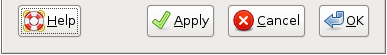
\includegraphics[height=15mm]{images/widget-keyboard-focus.png}
\caption{Billentyűzet fókusz jelzése a \textit{widget}en}
\end{center}
\end{figure}

Az egyes \textit{widget}ekre külön-külön engedhető, vagy tiltható a fókuszba kerülés, a \textit{can-focus}\index{GtkWidget@\texttt{GtkWidget}!tulajdonságok!can-focus@\texttt{can-focus}} tulajdonság állításával. Az egyes \textit{widget} típusok setében azonban ez az érték alapértelmezés szerinti értéke megfelel a céljainknak\footnote{Ez az érték egy \texttt{GtkEntry} esetén igaz, míg egy \textit{Gtkabel} esetén hamis alapértelmezés szerint.}. Ha kódból szeretnénk átmozgatni a fókuszt az egyik \textit{widget}ről a másikra, vagy csak azt kívánjuk elérni, hogy az ablak megjelenítésekor legyen olyan \textit{widget} ami fókuszban van, akkor a \texttt{grab\_focus} függvényt kell alkalmaznunk, aminek előfeltétele a \textit{can-focus} igaz értéke, azaz fókuszálhatónak kell lennie, ami viszont bizonyos \textit{widget}ek (pl.: \texttt{GtkFrame}) esetén nem értelmezett.

\subsubsection{Alapértelmezett \textit{widget}}

A \texttt{GtkWindow} estén -- amit rendszerint olyan ablakhoz használunk aminek nincsenek gombjai -- ritkábban, míg \texttt{GtkDialog}\index{GtkDialog@\texttt{GtkDialog}} esetén csaknem mindig használt tulajdonság az alapértelmezett \textit{widget}, mely ellentétben a fókusszal inkább egy logikai tulajdonság, a felületre nem, csak a működésre van hatása. Egy ablakon belül -- nevéből is következően -- legfeljebb egy olyan \textit{widget} lehet, mely rendelkezik ezzel a tulajdonsággal, ez rendszerint a dialógus jóváhagyó (\textit{affirmative}\index{gomb!jóváhagyó}) gombja, jellemzően az \textit{Ok}\index{gomb!ok} gomb.

\begin{figure}[H]
\begin{center}
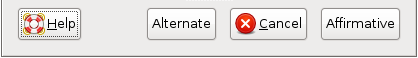
\includegraphics[height=15mm]{images/button-affirmative.png}
\caption{Gombok szokások sorrendje egy dialógusban}
\end{center}
\end{figure}

Hatása abban áll, hogy az alapértelmezett \textit{widget} -- vagyis ami esetén a \textit{can-default}\index{GtkWidget@\texttt{GtkWidget}!tulajdonságok!can-default@\texttt{can-default}} értéke igaz -- aktiválódik akkor, ha egy egysoros beviteli mező van fókuszban (\texttt{GtkEntry}\index{GtkEntry@\texttt{GtkEntry}}) és akkor \textit{Enter}t\index{billentyű!enter} nyomunk, ez is csak akkor, ha az \textit{entry} \textit{activates-default}\index{GtkEntry@\texttt{GtkEntry}!tulajdonságok!activates-default@\texttt{activates-default}} értéke szintén igaz értékű. Többsoros beviteli mező (\texttt{GtkTextView}\index{GtkTextView@\texttt{GtkTextView}}) esetén ez nem működőképes, hiszen ott az \textit{Enter} lenyomása soremelést jelent. Az alapértelmezett \textit{widget}nek a billentyűzetről való használat kényelmesebbé tételében van szerepe, hiszen ha minden szükséges mezőt kitöltöttünk egy dialógusban, akkor nem kell a megfelelő gombig -- egérrel, vagy \textit{Tab}\index{billentyű!tab} billentyű(k) lenyomásával -- elnavigálnunk, csak egyszerűen az \textit{Enter} leütésére aktiválódik az alapértelmezett \textit{widget}.

\subsection{Vezérlő elemek}
\label{sec:windowvsdialog}

Amennyiben a szükséges tartalmi elemeket elhelyeztük az ablakban, a vezérlő elemekkel is hasonlóan el kell eljárnunk. A különböző célokra használt ablakok különböző vezérlő elemeket kívánnak meg, amik az egyes típusokként erős hasonlóságot mutatnak. Egy főablak csak kivételes esetekben tartalmaz az eddigiekben tárgyalt gombokat, a vezérlés általában menükkel, a \textit{toolbar}on elhelyezett gombokkal történik (\ref{fig:windowprimary} ábra).

\begin{figure}[H]
\begin{center}
\subfloat[][Főablak]{\label{fig:windowprimary}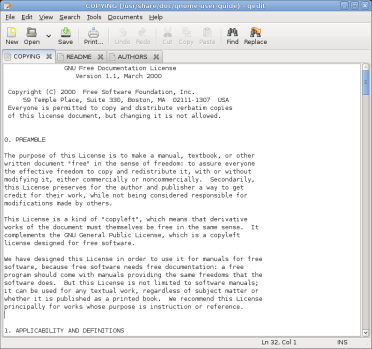
\includegraphics[height=60mm]{images/window-primary.png}}
\hspace{12pt}
\subfloat[][Dialógus]{\label{fig:windowdialogl}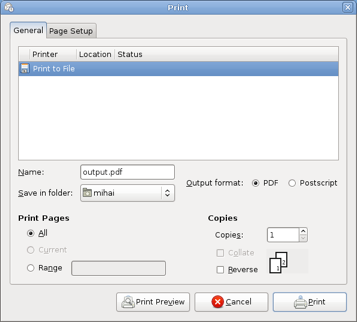
\includegraphics[height=60mm]{images/window-dialog.png}}
\caption{Tipikus ablakszerkezetek}
\end{center}
\end{figure}

A főablakból nyíló különböző célú ablakok, melyek például egy adott elem tulajdonságainak beállítására, egy bonyolultabb elem lépésenként történő felvételére, az alkalmazás egészének konfigurálására, egy folyamat nyomkövetésére, esetleg a felhasználó informálására, figyelmeztetésére szolgálnak, közvetlenül, vagy közvetve a \texttt{GtkDialog} típusból szármáznak, saját gombsorral látjuk el őket. Tipikus példa erre egy elem tulajdonságainak szerkesztésére használt dialógus (\ref{fig:windowdialogl} ábra).

\subsubsection{Dialog}
\label{sec:dialogbuttonadd}

A \textit{C} nyelvű változat mutat némi különbözőséget a \textit{C++} változattól a gombok hozzáadásának mikéntjében. Előbbi esetén ugyanis több gombot is hozzáadhatunk egyszerre a dialógoshoz, egymás után sorolva a \texttt{button\_text} és a \texttt{response\_id} paramétereket, majd a paraméterlistát, mindenképp \texttt{NULL} értékkel kell zárnunk, változatos programhibákkal fogunk szembesülni. Mindkét \textit{C} nyelvű függvény \texttt{button\_text} paramétere lehet vagy az általunk vágyott felirat szövege a gombon, vagy egy \textit{stock ID} (\textit{Ok} gomb esetén például \texttt{GTK\_STOCK\_OK}).

\lstinputsources
[numbers=none]
{sources/dialog_button_add.h}
{sources/dialog_button_add.hpp}
{Gomb hozzáadása \texttt{GtkDialog}hoz}
{lst:dialogbuttonaddh}

A \textit{C++} nyelvű változat működése sem tér el ettől jelentősen, hisz a \texttt{button\_text} itt is lehet \textit{stock ID} (\textit{Ok} gomb esetén például \texttt{Gtk::Stock::OK}), ami már csak ezért sem meglepő, mivel a \textit{StockId} típus egyik konstruktora \textit{Glib::ustring}et vesz át paraméterként.

\begin{figure}[H]
\begin{center}
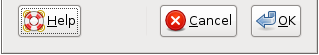
\includegraphics[height=13mm]{images/button-alternate.png}
\caption{Egy tipikus gombsor}
\end{center}
\end{figure}

A fenti elrendezésű -- amúgy meglehetősen szokványos -- gombsor az alábbi \textit{GTK+}, illetve \textit{gtkmm} kódrészlettel hozható létre.

\lstinputsources
[numbers=none]
{sources/dialog_button_add.c}
{sources/dialog_button_add.cc}
{Gomb hozzáadása \texttt{GtkDialog}hoz}
{lst:dialogbuttonadd}

\subsubsection{Message Dialog}
\label{sec:messagedialog}

Létezik a \textit{Dialog} típusnak egy -- a gombok hozzáadása szempontjából érdekes sajátossággal bíró -- specializált változata, melyet a felhasználóval történő kommunikáció céljaira használunk, s mely ennek megfelelően rendszerint csak az üzenet szövegét, illetve a válasz megadásához szükséges vezérlő elemeket tartalmazza.

\begin{figure}[H]
\begin{center}
\subfloat[][Információs üzenetablak]{\label{fig:messagedialoginformation}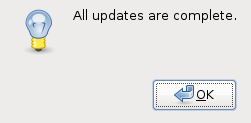
\includegraphics[height=30mm]{images/message-dialog-information.png}}
\hspace{12pt}
\subfloat[][Hiba üzenetablak]{\label{fig:messagedialogerror}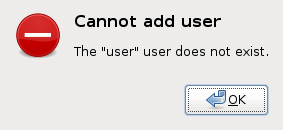
\includegraphics[height=30mm]{images/message-dialog-error.png}}
\caption{Tipikus üzenetablakok}
\end{center}
\end{figure}

Az ábrákon látható dialógusokat -- a szövegezéstől eltekintve -- csak típusuk különbözteti meg egymástól, s bal oldali (\ref{fig:messagedialoginformation}) egy információs ablak, míg a jobb oldali (\ref{fig:messagedialogerror}) egy hibadialógus. Az egyik szembeötlő különbség az ablakok között az ikon, amit az üzenetablak típusa határoz meg. A fenti két típuson kívül még két saját ikonnal rendelkező típus (\textit{question} és \textit{warning}) létezik, illetve készíthetünk ikon nélküli változatot, aminél módunk van saját ikon megadására.

Az üzenetablak típus eltérése, vagy inkább specialitása a \textit{dialog} típushoz képest nem csak a típus megadásának lehetőségére korlátozódik. A kifejezetten a szoftver és a felhasználó közötti ``üzenetváltás'' célját szolgáló \textit{widget} rendelkezik beépített elemekkel az üzenet megjelenítésére. A felhasználóval közölni kívántakat egy elsődleges és egy másodlagos (\texttt{primary-text}, \texttt{secondary-text}) részre bonthatjuk, ahol az előbbi egy rövid, csak a helyzet leglényegesebb elemit tartalmazó, egy mondatos összefoglalója a közölni kívánt információnak, vagy a javasolt kívánt műveletnek, míg az utóbbi ennek mélyebb, részletekbe menő kifejtése leírása, mely tájékoztatja a felhasználót a felmerült helyzet okairól, esetleges mellékhatásairól. Az esetek többségében a felhasználónak már az elsődleges szöveg elolvasását követően meg kell tudni hoznia döntését, a másodlagos szöveg a döntés alátámasztására, az esetleges kétségek eloszlatására szolgál.

A harmadik specialitás -- a gombok felhelyezésének mikéntje -- a vezérlő elemek szempontjából is említésre méltó. Azzal együtt, hogy \textit{dialog} típusnál ismertetett módszer az öröklődés okán természetesen itt is használható, de mivel a leggyakrabban használt gombkombinációk száma erősen korlátos, így azok közül -- a típussal együtt -- létrehozáskor választhatunk. Lehetséges értékek eredményeként vagy egyedüliként a \textit{Bezárás}, \textit{Ok}, \textit{Mégse} gombok, vagy a \textit{Ok}/\textit{Cancel}, \textit{Igen}/\textit{Nem} párosok kerülnek a dialógusra.

\lstinputsources
[numbers=none]
{sources/message_dialog_create.h}
{sources/message_dialog_create.hpp}
{\textit{MessageDialog} létrehozása}
{lst:messagedialogcreate}


A \textit{C} nyelvű változat, ellentétben a \textit{C++}-os megvalósítással nem egyetlen paraméterként várja az üzenetablak elsődleges szövegét, hanem egy \texttt{printf}-stílusú formátumleírót és az annak megfelelő paramétereket vesz át, amik típusbiztosságáról a \texttt{G\_GNUC\_PRINTF} makró gondoskodik, már amennyiben a \textit{GNU C} fordítót használjuk. Ebben az esetben fordítási idejű figyelmeztetést kapunk ha paramétereink nem felelnek meg a formátumleíróban megadottaknak.

\subsection{Megjelenítés}

Több lehetőség kínálkozik, ha egy ablakot, illetve annak tartalmát szeretnénk megjeleníteni. Használhatjuk egyrészről, a \textit{Widget}, a \textit{Window}, illetve a \textit{Dialog} típus által adott módszereket.

\subsubsection{Widget}

A korábban (\ref{par:widgetshow}) már tárgyalt \texttt{show} függvényt, ami megjeleníti a \textit{window}t, de csak a \textit{window}t, annak gyerekeit nem. Lévén a \textit{window} egy konténer típus, helyezhetünk el további \textit{widget}eket benne, amiknek a megjelenítéséről vagy már korábban gondoskodnunk kell -- mondjuk egy \texttt{show} hívással --, vagy megtehetjük a szülő és az összes gyerek megjelenítését egyszerre a \texttt{show\_all} (\ref{par:widgetshowall}) függvénnyel.

\subsubsection{Window}

Egy ablak esetén nem csupán a puszta megjelenítés lehet szempont, hanem az is, hogy a felhasználó az ablakot észre is vegye. Ez az estek túlnyomó többségében adott, hiszen valamilyen felhasználói interakció révén jelenik meg az új ablak. Ha viszont nem erről van szó akkor szükséges lehet az megjelenítésen túl más ablakok általi takarás megszüntetésére, a tálcáról való felhozatalra, az aktuális desktopra  történő mozgatásra, a fókusz (\ref{sec:widgetfocus}) átadására, mely műveletek mind függhetnek mind a platformtól, mind az ablakkezelőtől, mind pedig a felhasználói beállításoktól. Erre használható a \texttt{present} függvény.

\subsubsection{Dialog}

Egy \textit{window} típusú ablak esetén -- mivel jellemzően nincsenek az ablakon gombok és nem modálisak -- nincs igazán szükségünk arra, hogy -- a kód futásának szempontjából helyben -- kivárjuk a felhasználó reakciót. A \textit{dialog} típus ezzel szemben általában egy felhasználói interakció révén jelenik meg (pl.: egy elem tulajdonságait, vagy az applikáció beállításait szerkesztő ablak) és jelentős részben valamilyen döntés elé állítja a felhasználót (különösen igaz ez az üzenet ablakoknál, ahol kérést teszünk fel), melynek eredményéről szeretnénk értesülni. A \textit{dialog} típus \texttt{run} függvénye -- ahogy azt a következőekben (\ref{sec:dialogresponse}) részletesen is tárgyaljuk -- pontosan ezt a célt szolgálja. Egyrészről várakozik a felhasználó interakció -- amihez természetesen szükséges a \textit{main loop} futtatása -- majd visszatérési értékként az ablak ``futtatásának'' eredményét, vagyis a kiválasztott vezérlő elem -- az ablak elkészítésekor megadott -- \textit{response id}-t adja vissza. Mint látható, a függvény nem nem kifejezetten a dialógus megjelenítését szolgálja, az hasznos mellékhatásként mégis megtörténik.

\subsection{Bezárás}

A \textit{window} tehát leginkább a bezárás kapcsán állít kihívást elénk, melyet függően attól, mit szeretnénk elérni annak hatására, hogy a felhasználó az ablak bezárását kezdeményezte, több lehetséges megoldás, az egyes megoldásokra, pedig több módszer is kínálkozik.

\subsubsection{Blokkolás}

Kezdjük a legegyszerűbbnek látszó esettel, vagyis azzal, hogy semmilyen hatása ne legyen annak ha felhasználó az ablak bezárását kezdeményezi. Nyilván megfontolandó, hogy ezt tegyük, hiszen a felhasználó sem véletlenül akarja, amit akar, de ha mondjuk azt szeretnénk kikényszeríteni, hogy a főablakunkból csak a Fájl menüpont ``Kilépés'' almenüpontjára kattintva lehessen bezárni, akkor ez egy lehetséges megoldás\footnote{Ne becsüljük azonban alá se a felhasználói találékonyságot, se a felhasználói környezetek változatosságát. Semmiképp ne hagyatkozzunk arra, hogy egy adott módszer a felhasználó számára véleményünk szerint nem érhető el.}.

A feladat megoldása a korábban (\ref{par:widgetdeleteevent}) már tárgyalt \textit{delete-event} szignál kezelésében rejlik. Ahogy arról szó esett ez a szignál váltódik minden ablakon (\textit{toplevel window}), illetve minden az ablakban lévő \textit{widget}en, mikor a felhasználó az ablak bezárását kezdeményezi. A szignál két külön említésre is méltó sajátossággal is rendelkezik:

\begin{enumerate}
 \item A szignált kezelni kívánó függvénynek egy \textit{bool} értékkel kell visszatérnie, ami azt jelzi a \textit{GTK} felé, hogy az adott függvény kezelte-e az eseményt, egyszersmind nincs szükség a további kezelő függvény meghívására. A \textit{GTK} következésképp addig hívja sorra az szignálra ``feliratkozott'' függvényeket (\textit{signal handler}) -- köztük ha van ilyen, akkor az alapértelmezett szignálkezelő függvényt (\textit{default signal handler}) amíg egyikük \textit{true} értékkel nem tér vissza.
 \item Ha minden ilyen függvény \textit{false} értékkel tér vissza, azaz a szignál további propagálását kéri a \textit{GTK}-tól, akkor konkrétan a \texttt{delete-event} esetében a \textit{GDK} alapértelmezett eseménykezelője (\textit{default event handler}) fut le, ami meghívja az ablak destruktorát.
\end{enumerate}

Fentiek alapján ahhoz, hogy megelőzzük az ablak bezárását -- vagyis hogy ne történjen semmi -- el kell érnünk, hogy az alapértelmezett eseménykezelő ne hívódjon meg, azaz az általunk felkötött szignálkezelő \textit{true} értékkel kell hogy visszatérjen, jelezve azt, hogy az eseményt kezeltük, a további szignálkezelő függvények meghívására nincs szükség. Ebben az esetben ez azt is jelenti, hogy az alapértelmezett eseménykezelő sem hívódik meg. Ehhez definiálnunk kell a szignálkezelő  függvényeket, ami a korábbi (\lstref{lst:windowminimal}\footnote{A sorszámozás az eredeti példába való beillesztés pontját mutatja.}) példát kiegészítve az alábbihoz hasonló módon tehetünk meg,

\lstinputsources
[firstnumber=2]
{sources/window_persistent_callback.c}
{sources/window_persistent_callback.cc}
{Szignálkezelő függvény perzisztens ablakhoz}
{lst:windowpersistentcallback}

majd ezeket a függvényeket a \texttt{delete-event} szignálra be is kell kötnünk\footnote{A sorszámozás az eredeti példába való beillesztés pontját mutatja.}.

\lstinputsources
[firstnumber=12]
{sources/window_persistent_connect.c}
{sources/window_persistent_connect.cc}
{Szignálkezelő függvény bekötése perzisztens ablakhoz}
{lst:windowpersistentconnect}

Ha az adott szignál alapértelmezett szignálkezelő függvénnyel is rendelkezik -- ami a \textit{widget} osztály-leírójában kerül megadásra -- és magunk akarjuk a szignált kezelni, akkor szükségessé válik, hogy a saját kezelő függvényünk még az alapértelmezett előtt hívódjék meg, ami további praktikák bevetését igényli, amiről egy másik részben (\ref{par:defaultsignalhandler}) esik részletesebben szó.

Ha a saját szignálkezelő függvény írását kissé túlzónak találjuk egy olyan egyszerű feladat ellátására, mint egy \textit{true} értékkel való visszatérés, akkor akkor nem tévedünk, sőt a \textit{GTK+} fejlesztői is gondoltak erre és megalkották a \texttt{gtk\_true}, illetve a \texttt{gtk\_false} nevű függvényeket, melyek semmi egyebet nem tesznek, mint a nevüknek megfelelő értékkel térnek vissza, így a fenti példa szignálkezelő függvényei elhagyhatók, hiszen azok \textit{GTK+} által adott -- ekvivalens funkciójú -- függvényekkel helyettesíthetőek.

\lstinputsource
[language=C]
{sources/window_persistent_simple.c}
{Egyszerűsített szignálkezelő függvény bekötése}
{lst:windowpersistentsimple}

\subsubsection{Eltüntetés}

Folytassuk másodikként azzal az eshetőséggel, ha el szeretnénk tüntetni az ablakot, aminek a bezárását a felhasználó kezdeményezte. Az előző szituációhoz hasonlóan most is több módszer adódik a feladat megoldására.

A fent tárgyalt perzisztens ablakot eredményező szignálkezelők (\lstref{lst:windowpersistentcallback}) ismeretében a legnyilvánvalóbb megoldás, hogy még mielőtt visszatérnénk az adott függvényekből a \texttt{hide} függvény segítségével eltüntetjük az adott ablakot. A megoldás jó és működőképes megoldás lehet, ugyanakkor számolnunk kell azzal, hogy az ablak csak eltűnik, de nem feltétlenül semmisül meg. A már korábban is használt minimális példa azon kiegészítését is figyelembe vesszük, ahol a \texttt{delete-event} szignálra a \textit{main loop} futását megszakító függvényt hívjuk, akkor azt fogjuk tapasztalni, hogy az ablakunk eltűnik ugyan, de a mögöttes működés már nagyban attól függ a két implementációt (\ref{lst:windowminimalquit}., \lstref{lst:windowpersistentcallback}) miként vontuk össze. Ha a saját szignálkezelő függvényünket kötjük be előbb a \texttt{delete-event} szignálra, akkor az -- a visszatérési értéke révén -- leállítja a szignál további kezelését, vagyis a szignálkezelő függvények sorának meghívását is, így az ablak a saját kezelő függvényünk (\texttt{on\_delete\_event}), a \texttt{hide} hívással kiegészítve eltünteti az ablakot, de a következő szignálkezelő -- ami kiléptetné a \textit{main loop}ot -- már nem hívódik meg. Ha a felkötés sorrendje fordított, akkor előbb kilép a \textit{main loop} és csak ezután hívódik meg saját függvényünk, ami egyrészről elrejti az ablakot, másrészről blokkolja a további kezelést, aminek vésősoron nem lehet hatása, hiszen a \textit{main loop} már kilépett.

Amennyiben a célunk csupán az ablak eltüntetése egyszerűbben is elérhetjük ugyanezt, hiszen a \texttt{hide} függvény közvetlenül -- pontosabban egy beépített \textit{GTK+} keresztül -- is beköthető a \texttt{delete-event} szignálra. Ezt kényelmi funkciót a \textit{gtkmm} esetén elveszítjük -- hasonlóan az előző példához --, mivel az általunk használni kívánt szignálkezelő függvény deklarációja nem egyezik meg az előírttal, így tehát ezt a ``kényelmet'' a típusbiztosság oltárán fel kell áldozni.

\lstinputsource
[language=C]
{sources/window_hide_on_delete_event_simple.c}
{Egyszerűsített szignálkezelő függvény bekötése}
{lst:windowpersistentsimple}

Ha nem ragadunk le a könnyen érthető, ám nem túl életszerű minimális példánknál, akkor az mondható el, hogy ablakokat -- legyenek azok \textit{window}, vagy \textit{dialog} típusúak --, valamilyen felhasználói interakcióra reagálva hozunk fel, valamilyen kezelő függvényben. Az bezáráskori elrejtés akkor lehet hasznos számunkra, ha nem akarjuk újra és újrakonstruálni az ablakot az adott felhasználói műveletre. Erre lehet példa mondjuk egy névjegy (\textit{about}) ablak, aminek a tartalma nem változik a program futása során, így azt az alkalmazás indulásakor, vagy az első megtekintéskor létrehozzuk, utána már elegendő csak elrejteni, vagy újra megjeleníteni. Másik példa lehet egy státusz jellegű információkat megjelenítő ablak, amiben úgymond gyűjteni tudjuk az adatokat és ha a felhasználó be is zárja az ablakot, mi az elrejtés után az adatgyűjtést és az ablak tartalmának frissítését tovább fojtatjuk, majd az újbóli megjelenítéskor már a naprakész információk jelennek meg.

\subsubsection{Megszüntetés}

Mint az a fentiekből már kiderült -- függetlenül attól, hogy \textit{window}, \textit{dialog}, vagy ezekből származó típusokról van-e szó --, a \textit{delete-event} szignál kiváltódását -- ha egyebet nem teszünk -- az ablak destruktorának meghívás fogja automatikusan követni, ami az esetek túlnyomó többségében meg is felel a céljainknak.

\subsection{Eseménykezelés}
\label{sec:dialogresponse}

\subsubsection{Szinkron}

A \textit{dialog} és a \textit{window} típusok közötti eltérések (\ref{sec:windowvsdialog}) közül a legszámottevőbb -- mivel ehhez tartozik a legtöbb beépített szolgáltatás is --, a vezérlő elemek, más szóval a gombok kezelése. A \textit{dialog} nem csupán arra ad lehetőséget, hogy a gombokat egy erre a célra készült konténerbe helyezzük el -- ezt magunk is megtehetnénk minden különösebb erőfeszítés nélkül --, hanem az ezeken végzett felhasználói interakciókat is egyszerűen nyomon követhetjük. Választhatunk az adott (kód)környezetben számunkra kényelmesebb -- szinkron, illetve aszinkron eseménykezelés közül. Előbbi esetén helyben\footnote{Az ablak létrehozásának helyén.} tudjuk kezelni az eseményeket, utóbbi viszont eseménykezelő függvények megírását és bekötését teszi szükségessé.

\lstinputsources
{sources/dialog_minimal.c}
{sources/dialog_minimal.cc}
{Minimál példa \texttt{GtkDialog}hoz}
{lst:dialogminimal}

A \texttt{run} függvény (\ref{dialogminimalc:dialogrun}.) egyrészről függvényeket köt be a szükséges szignálokra (\texttt{response}, \texttt{unmap}, \texttt{delete-event}, \texttt{destroy}), majd egy saját \textit{main loop}ot futtatásán belül kezeli az említett eseményeket. Ha ezek közül bármelyik bekövetkezik, akkor a \textit{main loop} futása megszakad, és a \texttt{run} függvény a megfelelő értékkel visszatér. Ennek kezelése tipikusan egy \texttt{if}, vagy egy \texttt{switch} szerkezeten belül történik.

Ha a fenti minimális példát a korábbi, gombok hozzáadását tartalmazó forrással (\lstref{lst:dialogbuttonadd}) egészítjük ki\footnote{A változók deklarációinak hozzáadása szükséges a fordíthatóság érdekében.}, mondjuk az alábbihoz hasonló módon kezelhetjük a felhasználói döntés eredményeként kapott választ (\textit{response}).

\lstinputsources
[firstnumber=12]
{sources/dialog_run.c}
{sources/dialog_run.cc}
{Minimál példa \texttt{GtkDialog}hoz}
{lst:dialogrun}

Itt az egyszerűség kedvéért csak az \textit{Ok}, illetve a többi gomb kerültek megkülönböztetésre, így ha a \textit{Mégse}, illetve a \textit{Súgó} gomb aktiválódott, akkor is a \texttt{switch} szerkezet \texttt{default} ága (\ref{dialogrunc:switchcasedefault}) fut le. Kérdés azonban, hogy ha az imént megismert \texttt{delete-event} szignál váltódik ki az ablak bezáródásának hatására, annak mi lesz az eredménye. A válasz egyszerű, hiszen a \texttt{switch} első ágára (\ref{dialogrunc:switchcaseok}) nem futhatunk rá, tehát marad itt is a \texttt{default} ág. Ha külön szeretnénk kezelni ezt az esetet, akkor a \textit{C} változat esetén a \texttt{GTK\_RESPONSE\_DELETE\_EVENT}, a \textit{C++} esetén pedig a \texttt{Gtk::RESPONSE\_DELETE\_EVENT} konstans kezelésére kell egy új ágat beillesztenünk.

Nem minden esetet fedtünk azonban le, elképzelhető ugyanis, hogy a dialóg felszabadul, míg a \texttt{run} függvény fut. Ebben az esetben a visszatérési érték \texttt{RESPONSE\_NONE} lesz, így ezt az esetet is meg lehet különböztetni a többitől, azonban mégsem tanácsos. Helyette, ha mindenképpen meg akarjuk szakítani a \texttt{run} futását, akkor a \texttt{resposne} függvényt hívhatjuk, aminek eredményeként a \texttt{run} a \texttt{resposne}-nak paraméterként átadott értékkel tér vissza.

Az élelmesebbek megfigyelhetik, hogy \textit{dialog} példaprogramból (\lstref{lst:dialogminimal}) a \textit{window} hasonló példájához (\lstref{lst:windowminimal}) kimaradt a \texttt{show} függvény hívása, ami annak tudható be, hogy a \texttt{run} ezt megteszi helyettünk, ahogy a dialógusunkat is modálissá teszi a \texttt{run} futásának idejére.

\subsubsection{Aszinkron}

Ha valamilyen oknál fogva lemondanák a \texttt{run} adta kényelemről, lehetőségünk van az aszinkron kezelésre. Ebben az esetben a \texttt{run} helyett a \textit{show} függvényt hívjuk, illetve egy saját függvényt -- melyben elvégezzük a számunkra szükséges műveleteket -- kötünk be a \texttt{response} szignálra. Ezt a módszert használva ebben a függvényben kell gondoskodnunk az ablak felszabadításáról is, már amennyiben nem csak a \texttt{delete-event} esemény hatására szeretnénk, hogy ez megtörténjen. A \texttt{response} szignál paraméterei között a \texttt{response\_id} is szerepel, így a függvény tartalma hasonló lehet a \texttt{run} hívást követő kódhoz (\lstref{lst:dialogrun}). Működésben azonban van némi különbség, hiszen a \texttt{delete-event} alapértelmezett működésének megváltoztatására például nincs mód.

Az aszinkron a megoldásra lehet egy másik példa, ha a lehetséges választások mindegyike ugyanazzal az eredménnyel kell járjon, például be kell záródjon az ablak. Ennek olyan leginkább helyzetekben van realitása, ahol csupán egy (pl.: \textit{Bezárás}) gomb jelenik meg az ablakon. Erre lehet példa egy olyan üzenetablak (\textit{MessageDialog}), amiben nem egy kérdést teszünk fel, hanem csupán informáljuk a felhasználót.

\lstinputsource
[language=C]
{sources/dialog_destroy_on_response_simple.c}
{Egyszerűsített \textit{response}-kezelő függvény bekötése}
{lst:windowpersistentsimple}

\subsection{Saját eseménykezelő}

Ha a fentiekben vázoltak valamilyen oknál fogva nem elégítenék ki igényeinket, vagy már egyébként is alkalmasabb módszernek látszik egy saját \textit{widget} implementálása akkor nem kell egyebet tennünk, minthogy az ősosztály eseménykezelő függvényét felüldefiniáljuk a nyelvi változatnak megfelelő módon.

\lstinputsources
{sources/mywindow_part.c}
{sources/mywindow_part.cc}
{Eseménykezelő felüldefiniálása saját \textit{widget}osztályban}
{lst:mywindowpart}

A \textit{gtkmm} esetén ez egy lényegesen kisebb erőfeszítést igénylő feladat. Ahogy ezt a fenti kódrészlet is mutatja a \textit{C} változatból épp csak a leglényesebb részem elehető ki egy jó tucatnyi sorban\footnote{A teljes \textit{C} kód egy \ref{mywindowc:lastline} soros \texttt{.c}, illetve egy \ref{mywindowh:lastline} soros \texttt{.h} állományból áll.}, addig a csaknem teljes értékű \textit{C++} kód ennek a felét sem tesi ki.

\section{Platformfüggő sajátosságok}

Bár a \textit{GTK} -- a \textit{GDK}\footnote{GIMP Drawing Kit}, illetve a \textit{Glib} függvénykönyvtárakon keresztül -- komoly platformfüggetlenséget biztosít, mégis számolnunk kell a különbségekkel, különösen az ablakok kezelése kapcsán. Ezek közül itt csak a két legfontosabbat emeljük ki.

\subsection{Ablakkezelő}

Bizonyos értelemben maga a az ablakkezelő is egy platform, hisz ahogy az operációs rendszerek a tőlük elvárt funkciókat -- mint amilyen például a fájlkezelés -- a maguk módján valósítják meg, úgy az ablakkezelő rendszerek is saját szisztémájuk szerint teszik ezt. Bizonyos funkciók csak néhány ablakkezelő implementál, addig másokat csaknem minden ilyen rendszer megvalósít, bár arra nem számíthatunk, hogy az egyes megvalósítások minden részletben megegyeznek.

Az ablakkezelők különbözőségei fejlesztési oldalról azzal a következménnyel járnak, hogy a még akkor is szembe kell néznünk a platformosság okozta nehézségekkel, ha egyébként alkalmazásunkat nem használjuk több különböző\footnote{Ebben a tekintetben a \textit{Linux} alapú rendszereket közel azonosnak tekinthetjük} operációs rendszer alatt.

Még az olyan egyszerű és széles körben megvalósított funkciók kapcsán, mint amilyen maximalizálás, vagy a minimalizálás (\texttt{maximize}, \texttt{iconify}) kételkednünk kell a mögöttes implementáció meglétében, illetve figyelembe kell vennünk az egyes megvalósítások különbözőségeit, vagyis nem alapozhatunk ezen függvények meghívását követően arra, hogy az ablak abba az állapotba kerül, amire számítottunk. Akár az előbbiek említett funkciókra, akár mondjuk az ablak előtérben tartására (\texttt{keep\_above}), akár teljes képernyőméretre nagyításra (\texttt{fullscreen}), akár az összes munkaterület (\textit{desktop}) való egyszerre történő meg megjelenítésre (\texttt{stick}) kérjük az ablakkezelőt, nem bizonyos, hogy kérésünk teljesül. Ennek csak az egyik oka az, hogy az ablakkezelő nem támogatja az adott funkciót, a másik pedig, hogy kérésünket követően valaki más az előző, vagy éppen mindkettőtől eltérő állapot állít be. Ennél fogva ügyelnünk kell arra, hogy egy ilyen helyzetre programunk fel legyen készülve.

Az ablak dekorációja a másik olyan terület, ahol kéréseket (\textit{hint}) intézhetünk az ablakkezelő felé. Hasonlóan azonban a fent tárgyaltakhoz itt is igaz, hogy célszerű ellenőrizni feltételezéseinket arra vonatkozólag, hogy kérésünk úgy és abban a formában hajtódik végre, ahogy azt mi elgondoltuk. Számos olyan eset lehetséges az ablak dekorációján található bezáró gomb megjelenítésének tiltásától (\texttt{deletable}), az ablak \textit{taskbar}ból történő kihagyásáig (\texttt{skip\_takbar\_hint}) melynek implementációs részletei teljes egészében az ablakkezelőtől függenek.

\subsection{Vezérlő elemek}

A \textit{GTK} alapértelmezés szerint a gombokat a \textit{GNOME Human Interface Guideline}\cite{gnomehig} (\textit{HIG}) által javasolt elrendezését alkalmazza, vagyis a jóváhagyó (\textit{affirmative}\index{gomb!jóváhagyó}) gomb a jobb oldalon a szélső pozícióba kerül, míg a menekülő gomb (\textit{cancel}\index{gomb!menekülő}) ettől balra kerül. Ha eltérő -- úgymond alternatív elrendezést -- szeretnénk, akkor azt a \texttt{set\_alternative\_button\_order} függvény segítségével egy korábbi példát (\lstref{lst:dialogbuttonadd}) kiegészítve az alábbi módon állíthatjuk be.

\lstinputsources
[numbers=none]
{sources/dialog_button_order.c}
{sources/dialog_button_order.cc}
{Alternatív gombsorrend beállítása}
{lst:dialogbuttonorder}

Amennyiben az üzenetablakoknál megismert (\ref{sec:messagedialog}) páros gombok (\textit{Ok}/\textit{Cancel}, \textit{Igen}/\textit{Nem}) valamelyikét használjuk, akkor ezt a sorrendállítást a \textit{GTK} megteszi helyettünk.

\section{A kód}

A fenti példaprogramok \textit{C}/\textit{C++} nyelvű forrásfájljai a \textit{FLOSSzine}, azok egy részének eredeti változata pedig a \textit{GTK+}, illetve a \textit{gtkmm} érhetőek el az alábbi címeken.

\medskip
\noindent
\url{http://flosszine.org/hellow_window/sources}\\
\url{http://library.gnome.org/devel/gtk-tutorial}\\
\url{http://library.gnome.org/devel/gtkmm}

\subsection{Fordítás és linkelés}

A korábbiakhoz hasonlóan az alábbi parancssorok segítségével fordíthatóak programjaink.

\begin{lstlisting}[language=bash, numbers=none, basicstyle=\ttfamily, keywordsprefix=window, keywordstyle=\itshape, basewidth={0.5em, 0.4em}]
gcc gtk_source_file.c -o gtk_binary `pkg-config --cflags --libs gtk+-2.0`
g++ gtkmm_source_file.cc -o gtkmm_binary `pkg-config --cflags --libs gtkmm-2.4`
\end{lstlisting}

\subsection{Futtatás}

A futtatással ezúttal is a forrásfájlok -- egyszersmind a fordítás -- könyvtárában érdemes próbálkoznunk, a példaprogram nevétől függően a \texttt{./futtatható\_bináris} parancs kiadásával.

\subsection{Eredmény}

Bármily hihetetlen ezúttal sem történik semmi egyéb, mint az előző alkalommal. Remélhetőleg azonban a különbség mégis érzékelhető annyiban, hogy legutóbb a meglepetéssel teli borzongást ablakunk váratlan felbukkanása, míg most a bennünk szikraként felvillanó megértés okozza.

